\begin{figure}[H]
    \centering


    \tikzset{every picture/.style={line width=0.75pt}} %set default line width to 0.75pt

    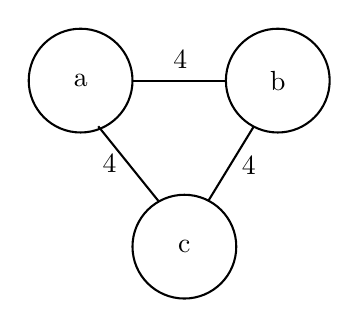
\begin{tikzpicture}[x=0.75pt,y=0.75pt,yscale=-1,xscale=1]
        %uncomment if require: \path (0,300); %set diagram left start at 0, and has height of 300

        %Shape: Circle [id:dp058849468526875004]
        \draw   (59,60) .. controls (59,46.19) and (70.19,35) .. (84,35) .. controls (97.81,35) and (109,46.19) .. (109,60) .. controls (109,73.81) and (97.81,85) .. (84,85) .. controls (70.19,85) and (59,73.81) .. (59,60) -- cycle ;
        %Shape: Circle [id:dp11003911798399524]
        \draw   (154,60) .. controls (154,46.19) and (165.19,35) .. (179,35) .. controls (192.81,35) and (204,46.19) .. (204,60) .. controls (204,73.81) and (192.81,85) .. (179,85) .. controls (165.19,85) and (154,73.81) .. (154,60) -- cycle ;
        %Shape: Circle [id:dp7927588085940704]
        \draw   (109,140) .. controls (109,126.19) and (120.19,115) .. (134,115) .. controls (147.81,115) and (159,126.19) .. (159,140) .. controls (159,153.81) and (147.81,165) .. (134,165) .. controls (120.19,165) and (109,153.81) .. (109,140) -- cycle ;
        %Straight Lines [id:da30216407066666995]
        \draw    (109,60) -- (154,60) ;


        %Straight Lines [id:da024128079077286868]
        \draw    (92.5,82) -- (121.5,118) ;


        %Straight Lines [id:da48310889364666654]
        \draw    (167.5,82) -- (145.5,118) ;



        % Text Node
        \draw (84,60) node  [align=left] {a};
        % Text Node
        \draw (179,60) node  [align=left] {b};
        % Text Node
        \draw (134,140) node  [align=left] {c};
        % Text Node
        \draw (132,50) node  [align=left] {4};
        % Text Node
        \draw (98,100) node  [align=left] {4};
        % Text Node
        \draw (165,101) node  [align=left] {4};


    \end{tikzpicture}

    \caption{Graph representation of both Table A and Table B}\label{fig:graph_limit_graph}

\end{figure}